\chapter{HANI Poroviscoelastic Characterization}\label{chap:5}

The Hybrid Hydrogels Augmented via Additive Network Integration (HANI) platform represents a novel approach to tissue engineering, specifically designed to address the complex mechanical requirements of meniscal tissue. By strategically integrating polycaprolactone (PCL) reinforcement networks within gelatin-based hydrogels, the HANI methodology creates composite scaffolds that combine the poroviscoelastic properties of hydrogels with the structural stability of thermoplastic reinforcement. While previous chapters have established the fabrication methodology, this chapter focuses on the comprehensive time-dependent mechanical characterization of these composite scaffolds.

Native meniscal tissue exhibits a unique set of mechanical properties that must be replicated by any viable replacement. These include appropriate stress response under compression, sustained load-bearing capacity, and viscoelastic behavior that facilitates energy dissipation during joint loading. The validation of static mechanical properties is therefore critical to assess whether HANI scaffolds can function effectively within the demanding mechanical environment of the knee joint.

The central research question addressed in this chapter is: Can PCL-reinforced gelatin hydrogels replicate the peak and equilibrium stresses of native meniscal tissue under quasi-static loading conditions? Furthermore, how do variations in crosslinking density and PCL reinforcement architecture influence these mechanical parameters across physiologically relevant strain levels?

\section{Experimental Design and Methodology}
\subsection{Hydrogel Formulation}
Two distinct gelatin-to-glutaraldehyde (GelA:GTA) mass ratios were selected for evaluation: 100:1 and 300:1. These formulations were chosen based on preliminary studies that demonstrated their capacity to maintain water content comparable to native meniscal tissue (approximately 76\%). The 100:1 ratio represents a higher crosslinking density expected to yield greater mechanical stiffness, while the 300:1 ratio provides a more compliant matrix with potentially enhanced fluid flow characteristics.

\subsection{PCL Reinforcement Configurations}
Four configurations were systematically evaluated to assess the impact of reinforcement architecture on mechanical performance:
\begin{itemize}
    \item \textbf{No PCL (Control)}: Hydrogel-only samples serving as baseline controls
    \item \textbf{Aligned PCL}: Linear PCL fibers with radial tie fibers for enhanced stability
    \item \textbf{Circumferential PCL}: Aligned fibers with additional circumferential bands to mimic the native meniscal collagen organization
    \item \textbf{3D PCL}: Thermomolded networks spanning the full hydrogel thickness to provide comprehensive three-dimensional reinforcement
\end{itemize}

\begin{figure}[H]
    \centering
    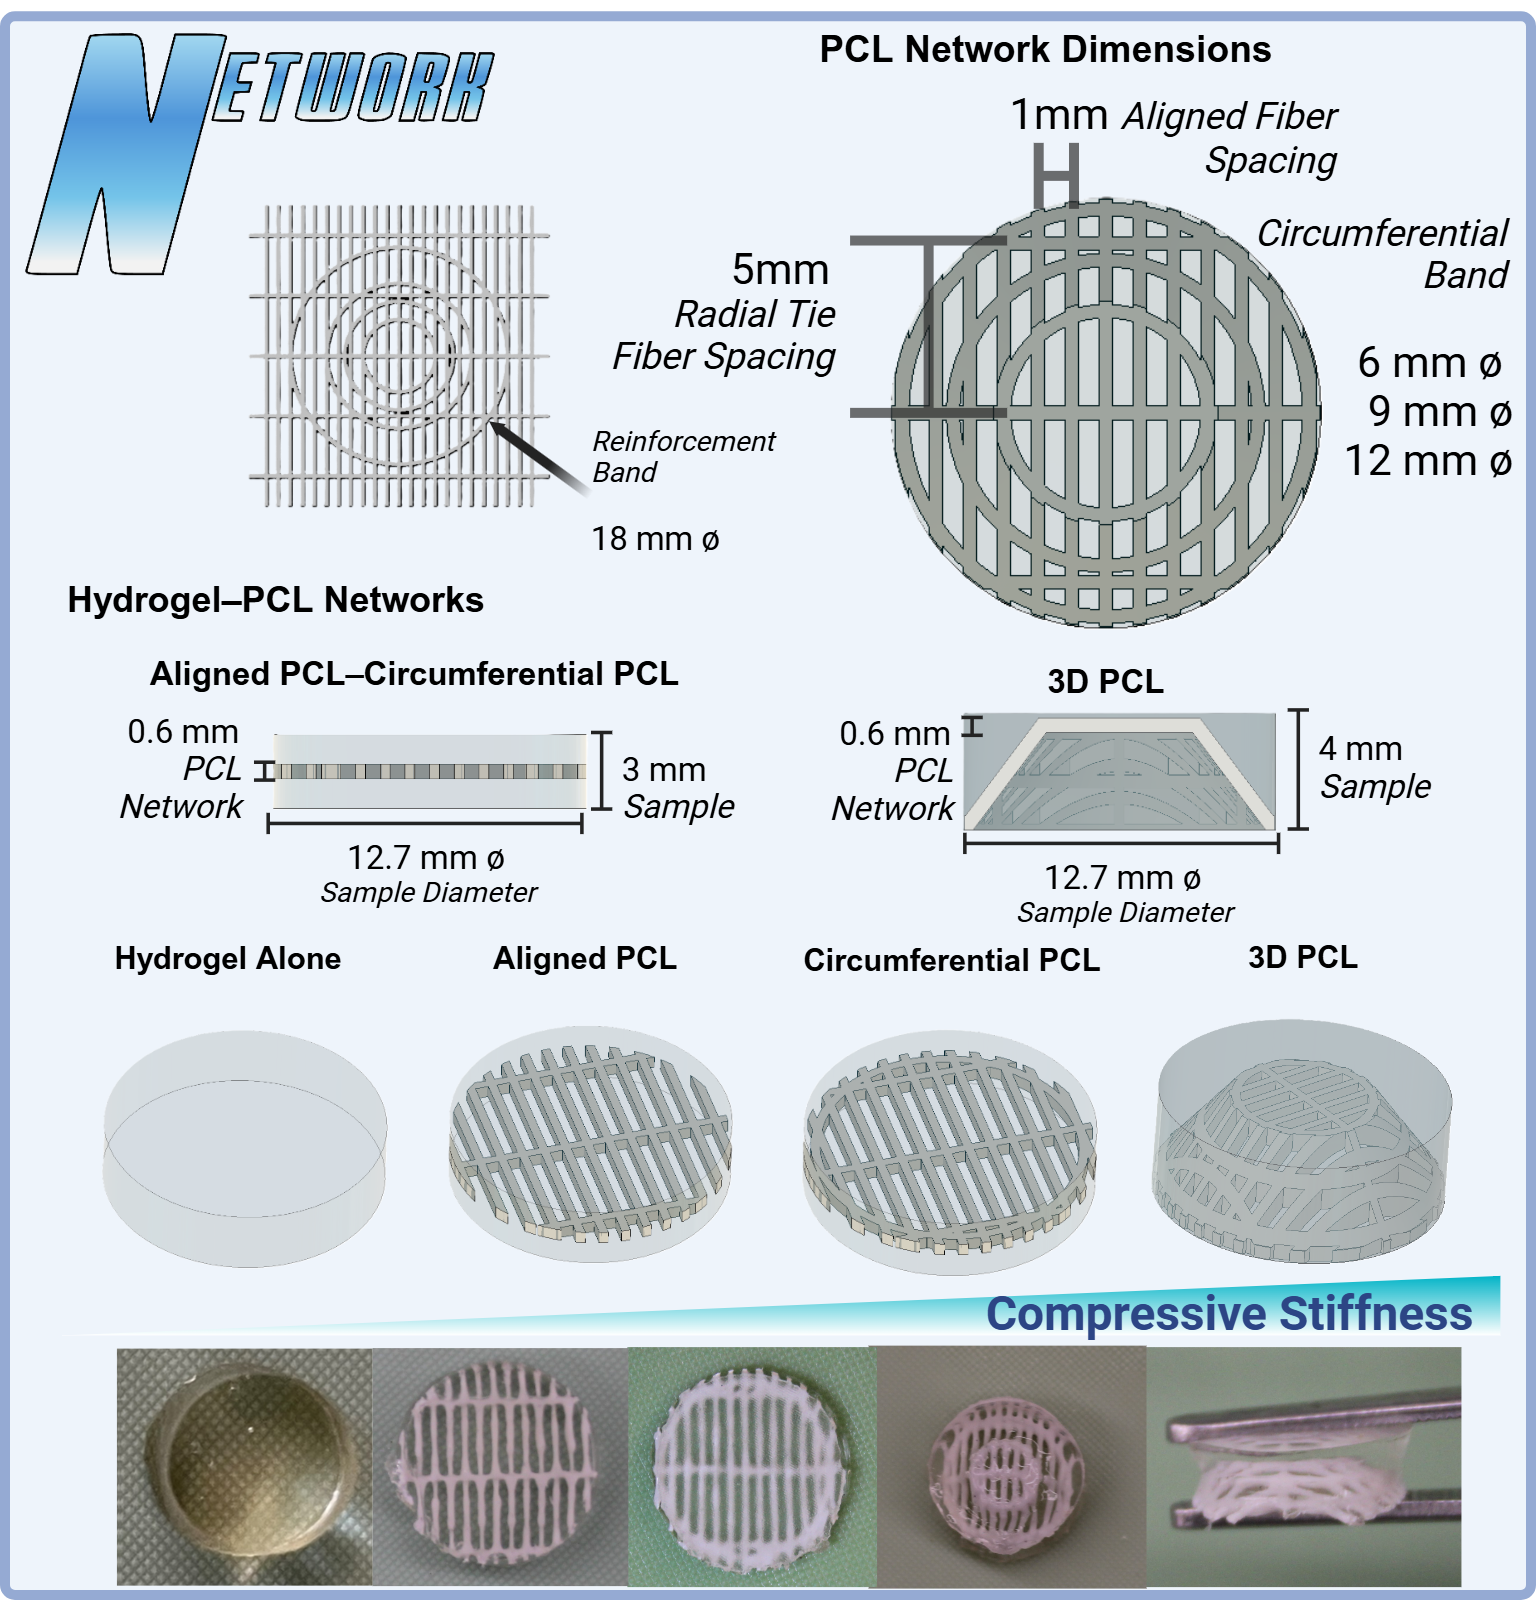
\includegraphics[width=1\linewidth]{figures/chapter_5/ch5_networks.png}
    \caption{Overview of engineered hydrogel–PCL composite architectures for poroviscoelastic evaluation. Top: schematic representations of circular and linear PCL network designs highlighting fiber alignment, circumferential reinforcement bands, and radial tie spacing. Dimensions were standardized for sample fabrication with outer diameters of 6, 9, and 12 mm. Middle: cross-sectional schematics of composite constructs—aligned-circumferential PCL networks (3 mm thickness) and thermomolded 3D PCL scaffolds (4 mm thickness)—embedded in gelatin hydrogel matrices. Bottom: representative samples of each construct group (Hydrogel Alone, Aligned PCL, Circumferential PCL, and 3D PCL) prepared for compressive stiffness testing. Insets display uniaxial loading conditions used to quantify mechanical response under physiologic strain.}
    \label{fig:ch5_networks}
\end{figure}

\begin{figure}[H]
    \centering
    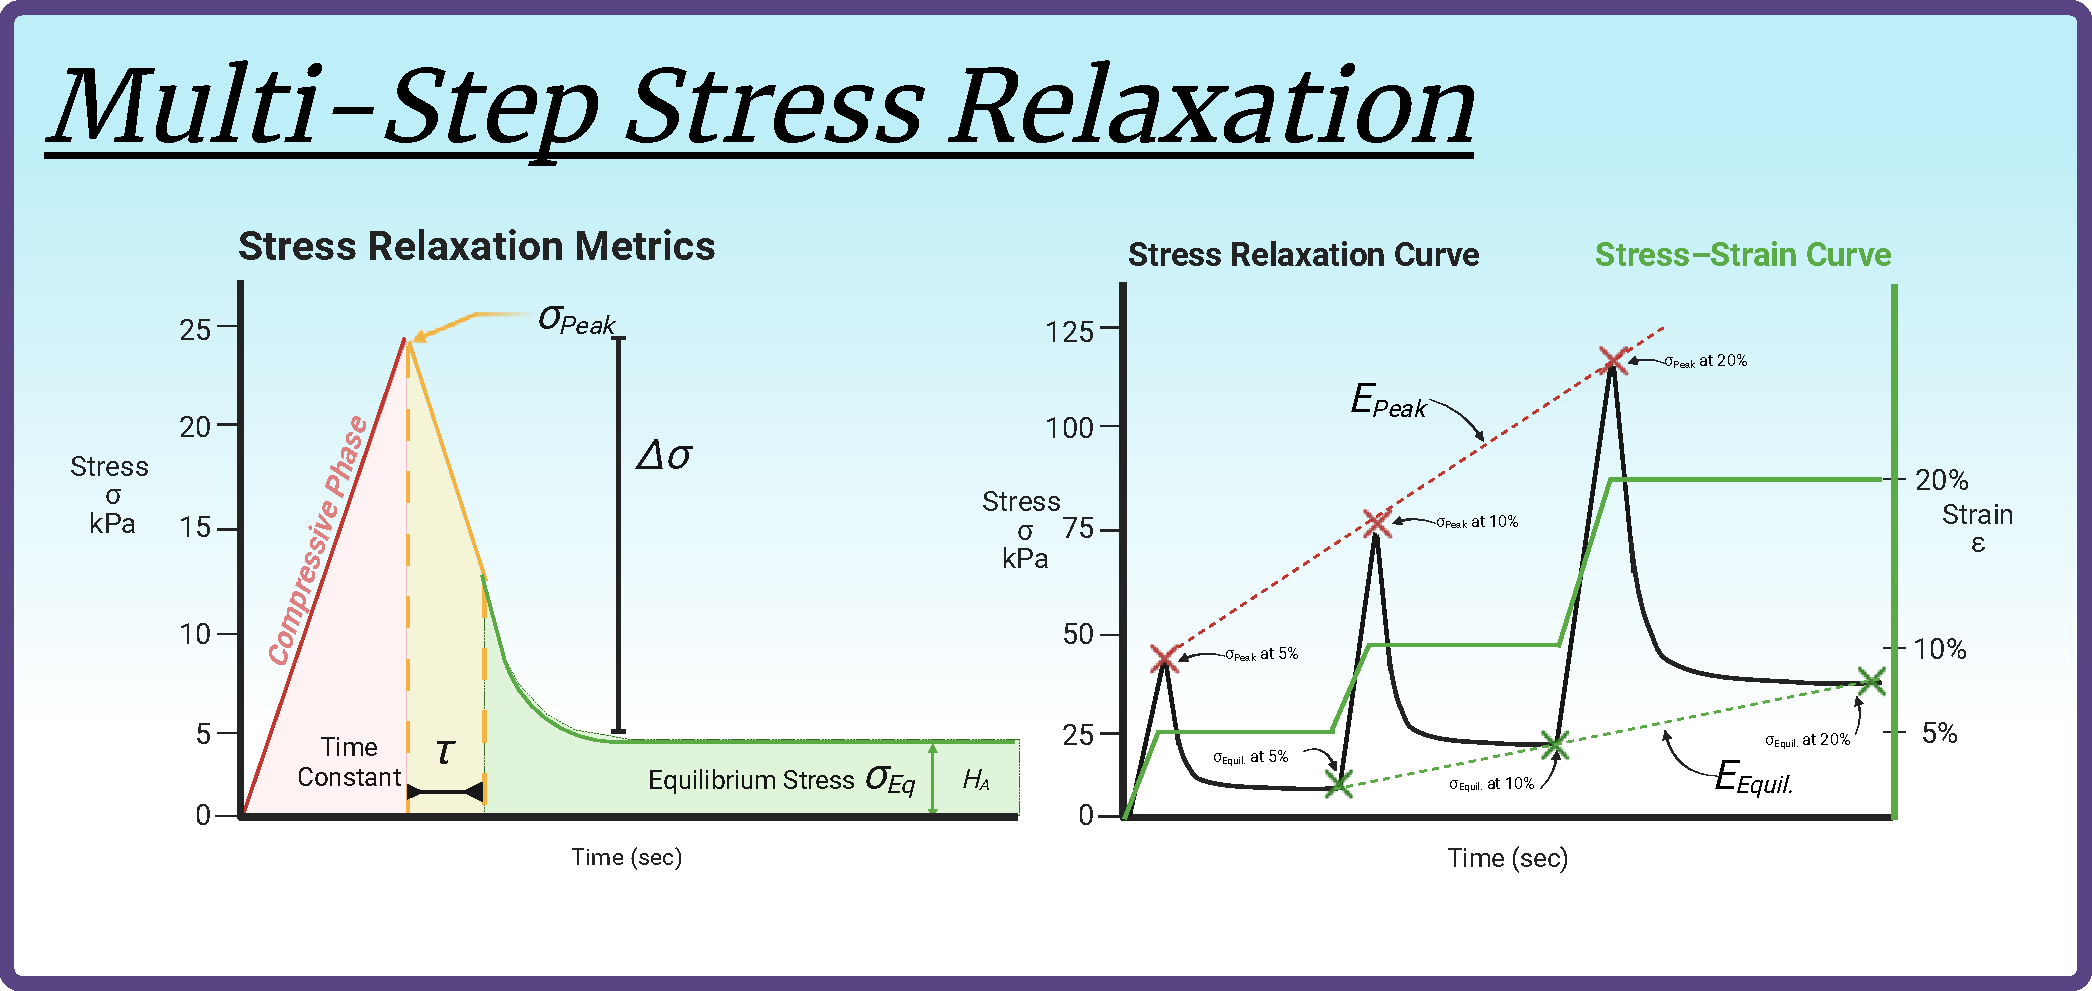
\includegraphics[width=1\linewidth]{figures/chapter_5/ch5_stressRelax.pdf}
    \caption{Schematic and experimental setup for confined compression stress-relaxation testing of hydrogel–PCL composite scaffolds. Samples were compressed to a fixed strain and held under deformation while force decay was recorded over time. This setup enabled evaluation of time-dependent mechanical behavior, including instantaneous modulus, equilibrium stress, and viscoelastic recovery profiles.}
    \label{fig:ch5_stressRelax}
\end{figure}

\subsection{Stress-Relaxation Testing Protocol}

To characterize the time-dependent mechanical performance of the HANI scaffolds, samples were subjected to a confined compression stress-relaxation protocol. This method enables quantification of viscoelastic behavior, simulating how the scaffold would respond to sustained loading in vivo. 

Each sample was placed in a confined chamber and compressed to a defined strain level. The deformation was held constant while the resulting stress decay was recorded over a specified duration. This allowed for the separation of instantaneous (elastic) response from long-term (viscous) behavior, providing both an initial modulus and an equilibrium stress value for each scaffold type.

By analyzing these parameters across scaffold designs—including hydrogel-only, aligned PCL, circumferential PCL, and 3D thermomolded constructs—comparisons could be drawn regarding their capacity to resist deformation, dissipate load, and recover over time. These findings offer critical insights into scaffold suitability for mimicking native meniscal poroviscoelasticity and guiding future design refinements.

The protocol consisted of:
\begin{itemize}
    \item Preload of 0.15 N for 1 minute to establish consistent initial conditions
    \item Stepwise compression to 5\%, 10\%, and 20\% strain
    \item Hold periods of 30 minutes at 5\% and 10\% strain, and 60 minutes at 20\% strain
    \item Continuous force and displacement recording throughout the test
\end{itemize}

\subsection{Stress Relaxation Behavior and Curve Fitting}
To further characterize the poroviscoelastic properties, stress relaxation data from each strain level were fitted to a single-phase logarithmic decay model in Python 3.9 using the following stress decay equation:

\begin{equation}
\textit{} \,\ \sigma(t) = \Delta \sigma e^{-t / \tau} + \sigma_{\text{\textit{Eq}}}
\end{equation}

\noindent Where $\sigma_{0}$ represents the peak stress at the start of constant strain hold immediately following compression (t = 0), $\Delta\sigma$ is the initial decay stress equal to the difference between initial peak stress and equilibrium stress, $\tau$ is the relaxation time constant, and $\sigma_{Eq}$ denotes the equilibrium stress measured at the end of each hold phase. The relaxation time constant $\tau$ quantifies how quickly the stress dissipates under constant strain, reflecting the scaffold's ability to redistribute mechanical forces—an essential feature for load-bearing tissues.

\section{Mechanical Parameter Definitions}
To facilitate systematic analysis of the stress-relaxation data, several key mechanical parameters were defined and calculated:

\subsection{Peak Stress ($\sigma_0$)}
The maximum stress recorded immediately upon reaching the target strain, representing the scaffold's instantaneous response to compression:
\begin{equation}
\sigma_0 = \frac{F_{\max}}{A}
\end{equation}
where $F_{\max}$ is the maximum force recorded and $A$ is the cross-sectional area of the sample.

\subsection{Equilibrium Stress ($\sigma_{Eq}$)}
The stress measured after relaxation has plateaued, indicating the scaffold's capacity for sustained load-bearing:
\begin{equation}
\sigma_{Eq} = \frac{F_{eq}}{A}
\end{equation}
where $F_{eq}$ is the equilibrium force after the hold period.

\subsection{Stress Decay ($\Delta\sigma$)}
The difference between peak and equilibrium stress, reflecting the scaffold's viscoelastic behavior:
\begin{equation}
\Delta\sigma = \sigma_0 - \sigma_{Eq}
\end{equation}

\subsection{Time Constant ($\tau$)}
A measure of the rate of stress relaxation, derived from fitting the stress-time curve to a single-phase exponential decay model:
\begin{equation}
\sigma(t) = \Delta\sigma \cdot e^{-t/\tau} + \sigma_{Eq}
\end{equation}

\subsection{Aggregate Modulus ($H_A$)}
The equilibrium stiffness under confined compression, calculated as:
\begin{equation}
H_A = \frac{\sigma_{Eq}}{\varepsilon}
\end{equation}
where $\varepsilon$ is the applied strain.


\subsection{Peak Modulus}
The peak modulus $(E_{peak})$ quantifies the material's instantaneous stiffness during the initial loading phases. To determine the peak modulus, the peak stresses at strain levels ($\varepsilon$ = 5\%, 10\%, 15\%(average) and 20\%) are plotted against the corresponding strains, and the slope of the linear regression line represents the peak modulus:

\begin{equation}
\textit{} \ E_{peak} = \frac{\Delta\sigma_{\text{\textit{0}}}}{\Delta\varepsilon}
\end{equation}

\noindent The peak modulus reflects the scaffold's resistance to deformation under compressive loads, with a higher slope indicating stiffer hydrogels. The peak modulus is essential for evaluating whether the HANI hydrogels provide the necessary mechanical integrity to handle dynamic joint stresses.

\subsection{Equilibrium Modulus Calculation}
The equilibrium modulus ($E_{Eq}$) measures the stiffness of the material at equilibrium, once internal fluid flow has ceased. This modulus is particularly relevant for biological tissues such as cartilage and menisci, where maintaining structural integrity under sustained loads is crucial for long-term functionality (Makris et al., 2011; Sanchez-Adams and Athanasiou, 2009). During stress relaxation testing, equilibrium stresses $\sigma_{Eq}$ are recorded at the end of each hold phase.
\begin{equation}
 \  E_{Equil}=\frac{\Delta\sigma_{Eq}}{\Delta \varepsilon}
\end{equation}


\section{Results}
\subsection{Compressive Stress Parameters}

\subsubsection{Peak Stress ($\sigma_0$)}
Increased crosslinking density and circumferential PCL reinforcement led to the greatest improvements in peak stress, particularly under high strain conditions. The 100:1 GelA:GTA formulation with circumferential PCL reinforcement demonstrated the highest peak stress values across all strain levels, reaching approximately 80 kPa at 20\% strain. This represents an eight-fold increase compared to unreinforced hydrogels of the same formulation and nearly matches the lower range of native meniscal tissue.

\subsubsection{Stress Decay ($\Delta\sigma$)}
Preservation of appropriate stress decay mechanics is essential for energy dissipation during joint loading. The integration of PCL networks significantly increased the magnitude of stress decay while maintaining physiologically relevant decay rates. This enhancement indicates improved capacity for shock absorption and load distribution, critical functions of native meniscal tissue.

\subsubsection{Equilibrium Stress ($\sigma_{Eq}$)}
The equilibrium stress followed similar trends to peak stress, with reinforced samples maintaining significantly higher stress levels after relaxation compared to unreinforced controls. Circumferential and 3D PCL configurations in the 100:1 GelA:GTA matrix exhibited the most substantial improvements, suggesting enhanced load-sharing between the hydrogel and PCL networks during sustained compression.

\subsubsection{Aggregate Modulus ($H_A$)}
The aggregate modulus, representing equilibrium stiffness, showed marked enhancement with PCL reinforcement. Values for circumferential and 3D PCL reinforcement in 100:1 GelA:GTA hydrogels approached 150 kPa, placing them within the range reported for native meniscal tissue. This finding confirms that strategic PCL reinforcement can effectively elevate the intrinsic mechanical properties of gelatin hydrogels to physiologically relevant levels.

\subsubsection{Time Constant ($\tau$)}
Remarkably, the time constant remained relatively consistent across PCL configurations, suggesting that scaffold damping behavior continues to be governed primarily by the hydrogel phase. This preservation of the hydrogel's intrinsic viscoelastic dynamics, despite substantial reinforcement, mirrors native poroviscoelastic behavior and indicates that fluid flow mechanisms remain functional within the composite structure.

\section{Results and Discussion}

This study introduced a novel method of hydrogel augmentation via the HANI method to mimic the native meniscus by leveraging the poroviscoelastic properties of gelatin-based hydrogels and the structural reinforcement of polycaprolactone (PCL). To achieve physiologically relevant properties, various mass ratios of gelatin to glutaraldehyde (GTA) were evaluated for water content, with the goal of approximating the native meniscus, which exhibits a water content of approximately 76\%. The 100:1 and 300:1 gelatin to GTA mass ratios were selected for further study as they closely matched native meniscal water content but albeit with slightly higher values (Figure 2). This adjustment was intentional, given the plan to incorporate PCL reinforcements, which would increase overall polymer content and modulate water retention.\\[0pt]

\indent Although differences in water content between formulations were not statistically significant, mechanical performance testing revealed substantial variations in load-bearing capacity, compressive stiffness, and stress relaxation behavior. Consequently, the 100:1 and 300:1 gelatin to GTA mass ratios were chosen to further assess the scaffolds' mechanical attributes across various PCL configurations.\\[0pt]

\indent The optimization process further involved integrating PCL reinforcement configurations (aligned, circumferential, and 3D) to enhance anisotropic load distribution, energy dissipation, and structural integrity under dynamic physiological forces. This synergy between chemical and mechanical properties positions the scaffolds as robust candidates for meniscal tissue engineering, demonstrating the potential to withstand repetitive joint loading while maintaining functionality over time \cite{norberg2021viscoelasticequilibrium}.

\begin{figure}[H]
    \centering
    \includegraphics[width=1\linewidth]{figures/chapter_5/graphs1.png}
    \caption{Effect of GelA-GTA mass ratio and PCL Reinforcement Type on Hydrogel Mechanical Properties Across Strain Levels. Bar graphs display peak stress ($\sigma_0$), stress delta ($\Delta\sigma$), and equilibrium stress ($\sigma_{Eq}$) for composite hydrogels with varying GelA-GTA mass ratios (300 and 100) and PCL reinforcement types (no PCL, aligned PCL, circumferential PCL, and 3D PCL) across strain levels of 5\%, 10\%, and 20\%. Significant increases in mechanical properties are observed at higher strain levels, particularly in 100 GTA hydrogels with circumferential and 3D PCL configurations. Statistical significance is denoted by *$p < 0.05$, **$p < 0.01$, ***$p < 0.001$, and ****$p < 0.0001$.}\label{fig:Ch3_graph1}
\end{figure}

\subsection{Peak Stress ($\sigma_0$)}

Peak stress ($\sigma_0$), a measure of the maximum stress the material can sustain under load, exhibited substantial improvements with both increased glutaraldehyde (GTA) concentration and polycaprolactone (PCL) reinforcement (Figure 3). For 300 GTA hydrogels, unreinforced samples displayed modest peak stress values, reaching 2.45 ± 0.20~kPa at 5\% strain and 9.79 ± 2.47~kPa at 20\% strain. Aligned PCL reinforcement more than doubled these values, achieving 5.19 ± 1.50~kPa at 5\% strain and 44.13 ± 13.75~kPa at 20\% strain. Circumferential PCL reinforcement provided even greater improvements, with $\sigma_0$ reaching 7.25 ± 0.87~kPa at 5\% strain and 61.90 ± 20.01~kPa at 20\% strain. Similarly, 3D PCL scaffolds enhanced peak stress to 8.03 ± 1.82~kPa and 49.17 ± 13.17~kPa at 5\% and 20\% strain, respectively.

In 100 GTA hydrogels, peak stress values were markedly higher than 300 GTA hydrogels for most configurations, except the initial Aligned PCL which reported slightly lower values at 5\% and 20\% strains, due to the increased cross-linking density. Unreinforced samples exhibited peak stresses of 3.84 ± 0.60~kPa at 5\% strain and 27.63 ± 4.94~kPa at 20\% strain. Aligned PCL reinforcement further improved $\sigma_0$, reaching 5.65 ± 1.22~kPa at 5\% strain and 42.30 ± 11.82~kPa at 20\% strain. Circumferential PCL reinforcement achieved the highest values, with $\sigma_0$ increasing to 7.54 ± 1.50~kPa at 5\% strain and 79.38 ± 16.40~kPa at 20\% strain. The 3D PCL configuration also performed well, with peak stresses reaching 9.04 ± 0.11~kPa at 5\% strain and 56.16 ± 2.98~kPa at 20\% strain.

Two-way ANOVA revealed significant effects for strain level and PCL configuration for both GelA-GTA mass ratios on peak stress (p~< 0.0001). Post-hoc Tukey's tests confirmed that circumferential and 3D PCL configurations significantly outperformed aligned and unreinforced hydrogels (p~< 0.05). Among the configurations, circumferential PCL reinforcement in 100 GTA hydrogels yielded the highest peak stress values, highlighting its superior ability to distribute loads effectively.

These results underscore the importance of HANI's strategic PCL reinforcement, particularly circumferential and 3D configurations, in enhancing the mechanical strength of hydrogels. The highest peak stresses observed in circumferential PCL-reinforced 100 GTA hydrogels mimic the anisotropic properties of native meniscal tissue, indicating their potential as load-bearing candidates for orthopaedic applications \cite{MartinSeitz2013,Visser2015}.

\subsection{Stress Decay ($\Delta\sigma$)}

Two-way ANOVA revealed significant effects for both GelA-GTA mass ratios on strain level and PCL configuration for stress decay (p~< 0.0001), with circumferential and 3D PCL reinforcements significantly outperforming aligned and unreinforced hydrogels (p~< 0.05). These results indicate that strategic reinforcement, particularly circumferential PCL in a 100 GTA matrix, provides superior stress decay performance, enhancing resilience under prolonged compressive loading \cite{Patel2019,Morejon2020,Norberg2021,Roberts2011}.

\subsection{Equilibrium Stress ($\sigma_{Eq}$)}
These findings highlight the role of circumferential and 3D PCL reinforcements, particularly in 100 GTA hydrogels, in enhancing equilibrium stress. The ability to sustain higher stress levels over extended periods reflects the potential of these configurations to mimic the load-bearing behavior of native meniscal tissue, making them promising candidates for meniscal replacement applications \cite{MartinSeitz2013,Maes2006,Korhonen2002,Boschetti2004,Norberg2021,Roberts2011}.

\subsection{Aggregate Modulus ($H_A$)}

The increased stiffness in 100 GTA hydrogels with circumferential and 3D PCL reinforcement closely mirrors the compressive properties of native human meniscal tissue, with aggregate modulus values ranging on the order of 100--150~kPa. These configurations demonstrate the durability and resilience required for long-term orthopaedic applications, making them strong candidates for meniscal tissue engineering. HANI's combination of mechanical robustness and sustained compressive stiffness ensures both immediate load support and enduring performance under cyclic loading conditions \cite{Athanasiou2009,MartinSeitz2013,Patel2019,Morejon2020,Morejon2022,Bahcecioglu2019,Cakmak2020,Hernandez2017}.

\subsection{Time Constant ($\tau$)}

The time constant ($\tau$), indicative of the time required for hydrogels to reach equilibrium stress, exhibited minimal variation across PCL reinforcement types, suggesting limited influence on viscoelastic relaxation properties (Figure 4). In 300 GTA hydrogels, $\tau$ values remained consistent across configurations, with circumferential and 3D PCL reinforcement showing slight decreases compared to unreinforced samples. Similarly, in 100 GTA hydrogels, $\tau$ values were slightly higher for circumferential and aligned PCL reinforcements but did not show substantial changes \cite{Vemaganti2020}.

The consistent $\tau$ values across strain level and PCL configurations indicate that PCL reinforcement enhances mechanical strength without significantly altering the gelatin matrix's intrinsic relaxation dynamics for both GelA-GTA mass ratios. Reinforcement primarily influenced mechanical parameters like peak and equilibrium stress, while preserving viscoelastic stability \cite{Vemaganti2020,Maes2006,Mirani2009}.

The negligible effect of PCL reinforcement on $\tau$ suggests that the hydrogels retain their natural damping properties essential for energy dissipation and shock absorption. These properties, combined with the mechanical benefits of PCL reinforcement, make hydrogels with circumferential and 3D PCL in a 100 GTA matrix particularly suitable for load-bearing applications like meniscal replacements \cite{Shemesh2014,Patel2019}.

\begin{figure}
    \centering
    \includegraphics[width=1\linewidth]{figures/chapter_5/graphs2.png}
    \caption{Effect of GelA-GTA mass ratio and PCL Reinforcement Type on Hydrogel Mechanical Properties Across Strain Levels. Bar graphs display time constant ($\tau$) and aggregate modulus ($H_A$) for composite hydrogels with varying GelA-GTA mass ratios (300 and 100) and PCL reinforcement types (no PCL, aligned PCL, circumferential PCL, and 3D PCL) across strain levels of 5\%, 10\%, and 20\%. Statistical significance is denoted by *$p < 0.05$, **$p < 0.01$, ***$p < 0.001$, and ****$p < 0.0001$.}\label{fig:Ch3_graph2}
    \end{figure}

\begin{figure}[H]
    \centering
    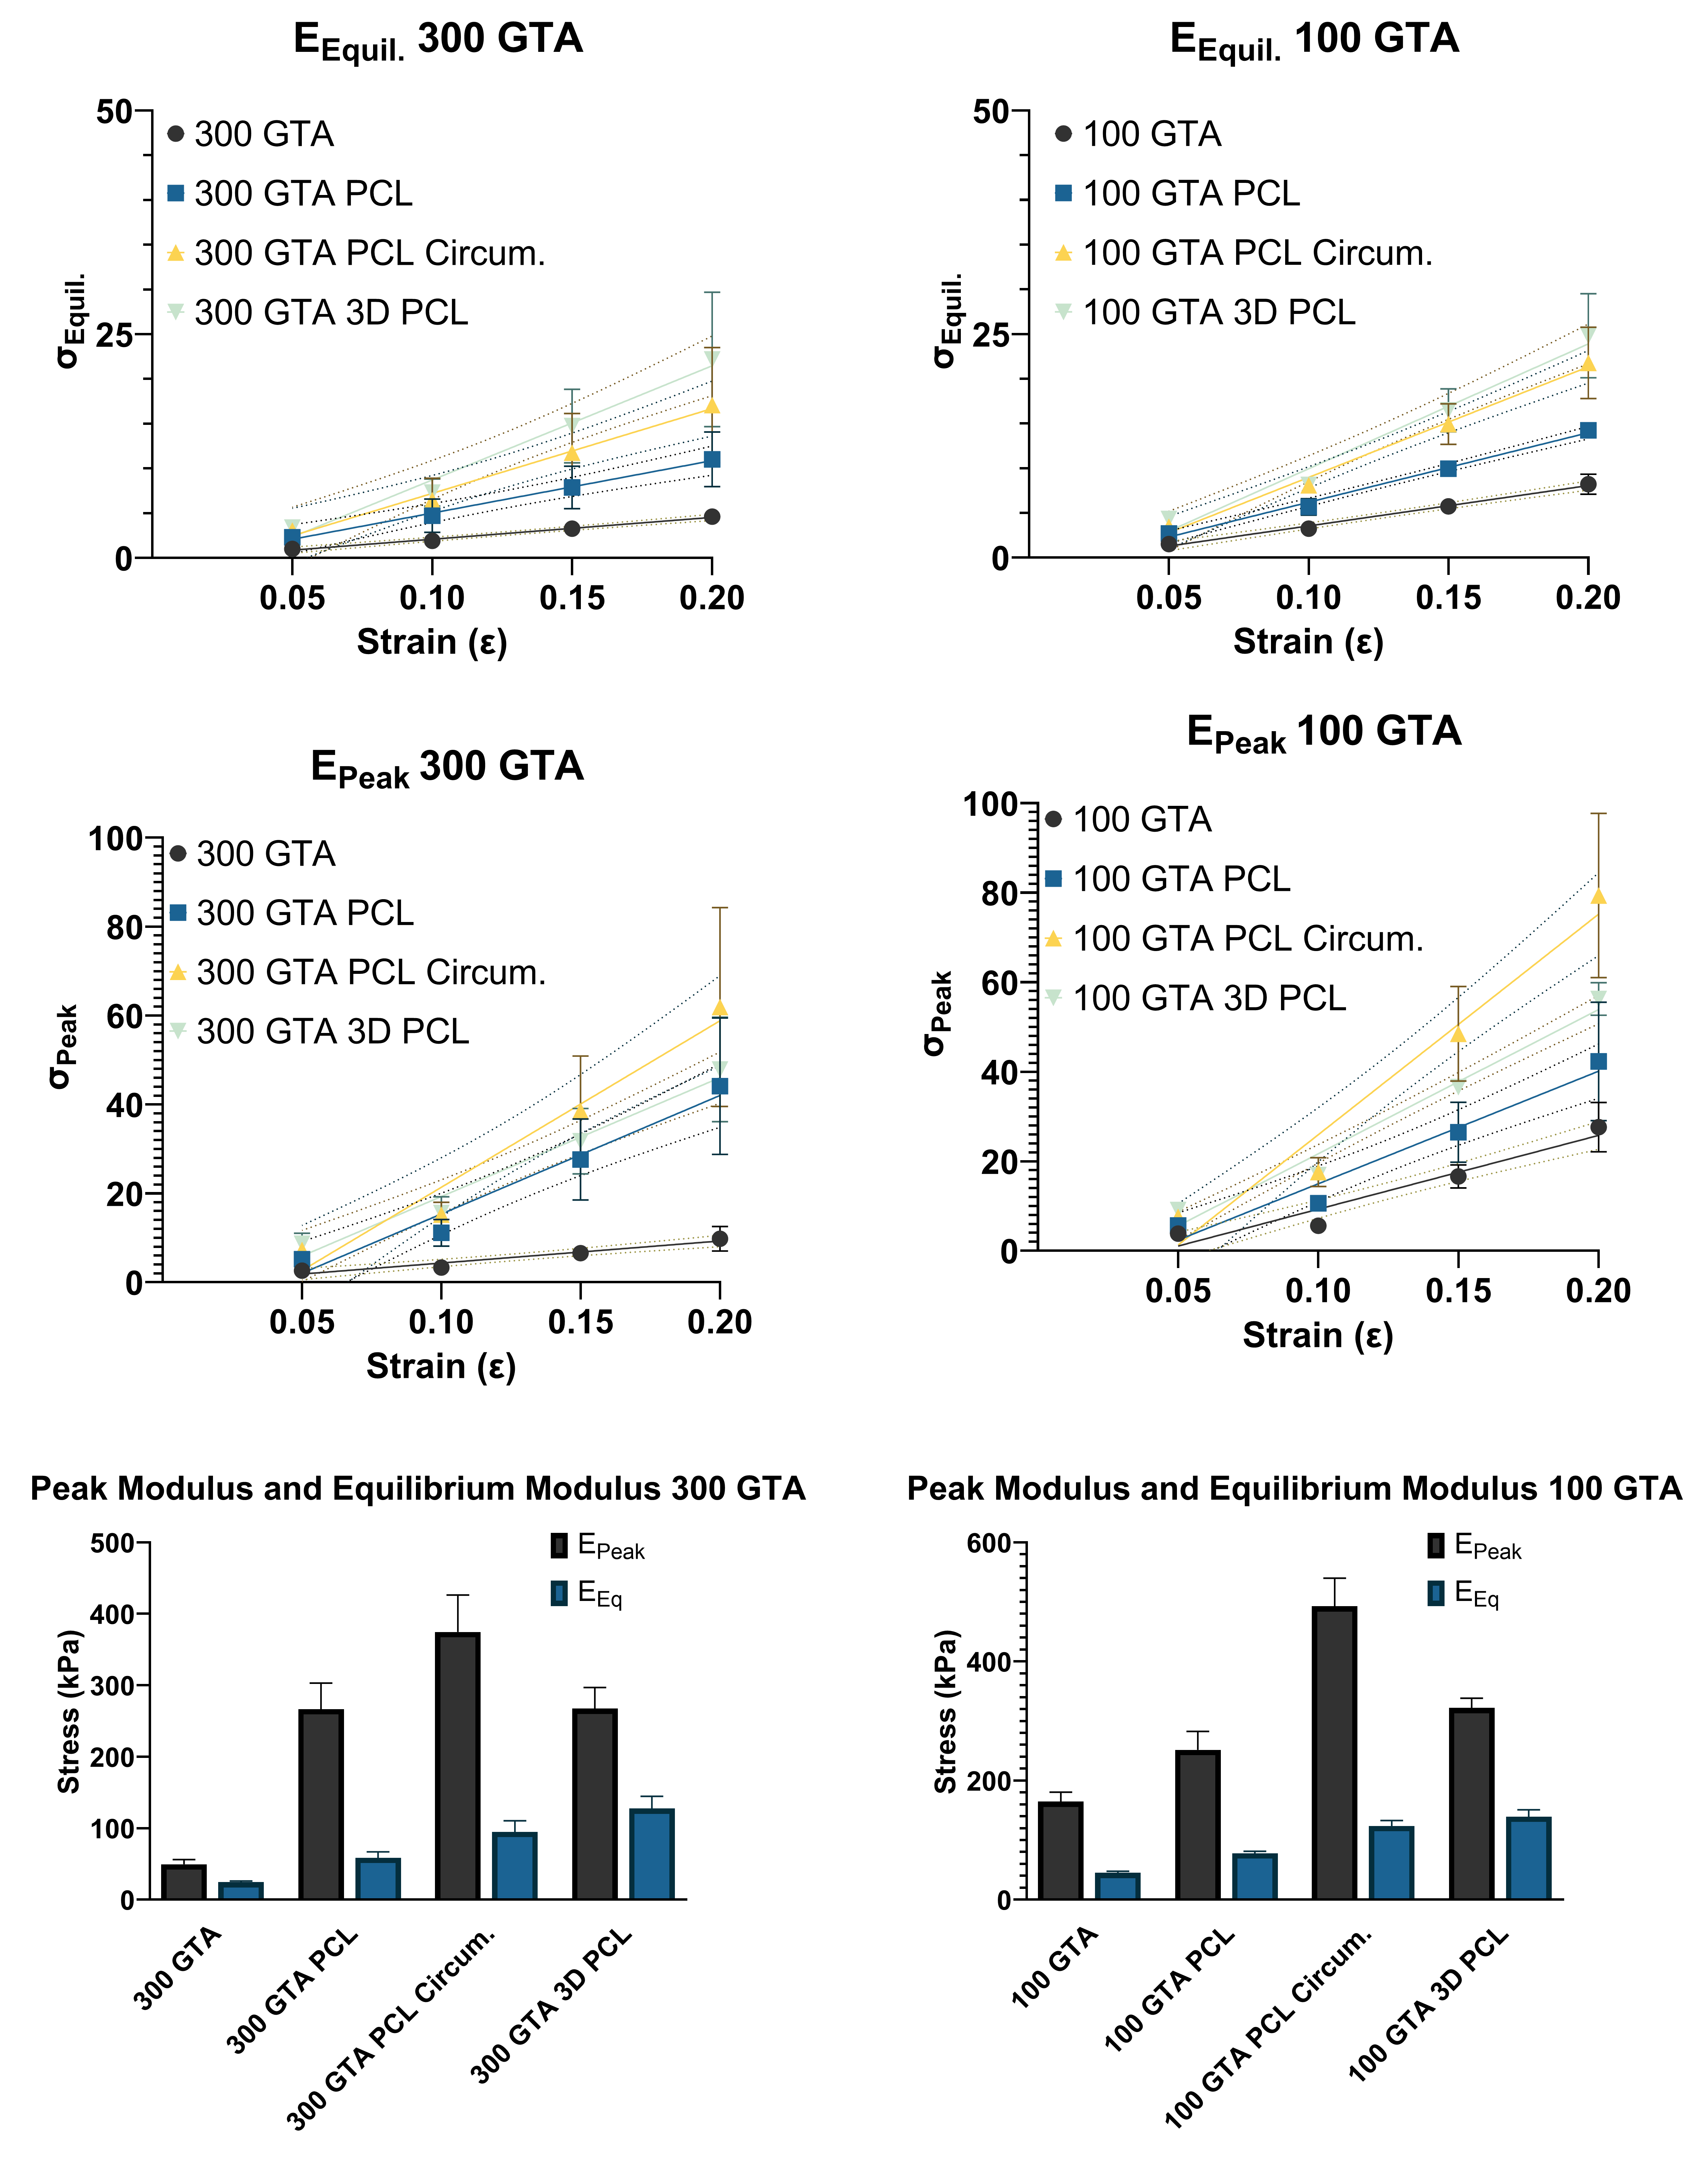
\includegraphics[width=1\linewidth]{figures/chapter_5/graphs3.png}
    \caption{Peak and Equilibrium Modulus Analysis of HANI Hydrogels with Varying GelA-GTA mass ratios, PCL Reinforcement Types, and Strain Levels. Line graphs in the top panels show peak and equilibrium moduli for HANI hydrogels formulated with 300 and 100 GelA-GTA mass ratios, with different PCL reinforcement types (no PCL, aligned PCL, circumferential PCL, and 3D PCL). The slopes of these lines correspond to the peak modulus ($E_{Peak}$), and equilibrium modulus ($E_{Equil}$). The bar graphs in the lower panels summarize the peak and equilibrium modulus values across the PCL configurations for each GelA-GTA mass ratio. Increased modulus values are noted in hydrogels with circumferential and 3D PCL configurations, particularly in the 100 GTA group, indicating superior mechanical reinforcement and resistance to deformation under strain. Error bars represent standard deviations. }
    \label{fig:Figure 5}
    \end{figure}

\subsection{Peak Modulus ($E_{peak}$)}

Peak modulus ($E_{peak}$), representing initial stiffness, increased significantly with for both GelA-GTA mass ratios across PCL reinforcements (\autoref{fig:Figure 5}). In 300 GTA hydrogels, unreinforced samples showed a peak modulus of 49.58 kPa, which improved with aligned PCL (266.60 kPa), circumferential PCL (374.60 kPa), and 3D PCL (267.60 kPa). For 100 GTA hydrogels, the unreinforced modulus of 164.80 kPa increased to 251.60 kPa with aligned PCL and peaked at 492.80 kPa with circumferential PCL. The 3D PCL configuration achieved 322.20 kPa, with a strong model fit (R² = 0.96). Linear regression confirmed significant effects for both GelA-GTA mass ratios across PCL reinforcements on peak modulus with all configurations having strong model fits ( R²>0.745,  p < 0.0001). 

The marked improvements in peak modulus with circumferential and 3D PCL configurations highlight their ability to distribute compressive forces effectively, especially in 100 GTA hydrogels. These enhancements align with the mechanical demands of meniscal tissue engineering, where high initial stiffness is critical for load-bearing applications \cite{31,59,60}.

\subsection{Equilibrium Modulus ($E_{Equil}$)}

Equilibrium modulus ($E_{Equil}$), indicative of stiffness under sustained loads, showed substantial increases for both GelA-GTA mass ratios for PCL reinforcement (\autoref{fig:Figure 5}). For 300 GTA hydrogels, the unreinforced modulus of 24.43 kPa rose to 58.59 kPa with aligned PCL, 94.79 kPa with circumferential PCL, and 127.60 kPa with 3D PCL. In 100 GTA hydrogels, circumferential PCL reached 123.60 kPa, while the highest value, 139.50 kPa, was recorded with 3D PCL.

Linear regression confirmed significant effects for both GelA-GTA mass ratios across PCL reinforcements on equilibrium modulus with all configurations having strong model fits ( R²>0.735,  p < 0.0001) with the exception of 300 GTA circumferential PCL (R²>0.672, p<0.0001). 

The high equilibrium modulus values achieved with circumferential and 3D PCL reinforcements in 100 GTA hydrogels highlight their ability to sustain loads effectively over time. These configurations mirror the sustained stiffness of native meniscal tissue, demonstrating strong potential for use in durable, load-bearing meniscal replacements \cite{21,60,61,62}.


\subsection{Design Implications}

HANI's scaffold design leveraged advanced additive manufacturing techniques, combining stereolithography (SLA) and fused deposition modelling (FDM). SLA was pivotal in producing precise molds that preserved alignment and stability of PCL reinforcements, enabling networks to span the scaffold's thickness and mimic the anisotropic properties of the native meniscus \cite{Filardo2019,Klarmann2023,Bahcecioglu2019,Coluccino2017}. FDM enabled continuous fiber printing, creating circumferential and radial-tie fibers that transformed axial compressive loads into tensile stresses. This reinforcement strategy, particularly in the 3D-PCL configuration, ensured progressive load sharing and minimized localized deformation. Together, these techniques produced scaffolds capable of mimicking the hoop stress-strain behavior of the native meniscus, absorbing and redistributing forces effectively to protect surrounding cartilage \cite{Filardo2019,Guo2021,Armiento2018,Visser2015}.

\subsection{Challenges and Limitations}

It is important to note that variability in PCL placement can occur as a result of molding and fiber misalignment during hydrogel integration; potentially affecting mechanical properties and construct reproducibility. Future developments of the HANI process will focus on optimizing these fabrication techniques to ensure consistent PCL distribution, including the improvement of mold designs and the introduction of thermal stabilization strategies. Additionally, standardizing fabrication protocols and implementing more precise quality control measures, such as real-time imaging during scaffold formation, may help mitigate these inconsistencies in future studies. While the current scaffold fabrication approach produces reinforced hydrogel constructs with improved short-term mechanical performance, long term degradation and in vivo stability remain unexplored. Future research will focus on assessing scaffold behavior under physiological conditions in both in vitro and in vivo settings. These studies will be essential to validate the scaffold's durability and clinical applicability for meniscal tissue engineering.

\section{HANI-Key Innovations}

In this study, a novel scaffold fabrication strategy---Hybrid Hydrogels Augmented via Additive Network Integration (HANI)---was developed to address the critical mechanical and biological challenges in meniscal tissue engineering. By integrating architecturally controlled polycaprolactone (PCL) networks within gelatin-based hydrogels, the HANI method successfully enhanced scaffold mechanical performance while preserving the poroviscoelastic behavior essential for mimicking native meniscal tissue.

Specifically, scaffolds reinforced with circumferential and three-dimensional (3D) PCL configurations exhibited substantial increases in peak stress, equilibrium stress, and aggregate modulus compared to hydrogel-only controls. Importantly, the intrinsic viscoelastic relaxation properties of the gelatin phase remained largely unaltered, indicating that mechanical reinforcement did not compromise time-dependent fluid flow behavior critical for joint function.

These findings demonstrate that the strategic integration of multi-directional PCL fibers can recapitulate the anisotropic load-bearing mechanisms of the native meniscus. Moreover, the use of additive manufacturing techniques such as stereolithography (SLA) and fused deposition modeling (FDM) allowed for precise spatial control over reinforcement architectures, paving the way for customizable, patient-specific implant fabrication.

\subsection{Key Innovation}

First demonstration of a hybrid scaffold platform combining tunable gelatin hydrogels with thermoformed, 3D PCL reinforcement networks.

\subsection{Performance Highlights}

Enhanced compressive mechanical properties while maintaining stress-relaxation behavior characteristic of native meniscus.

\subsection{Clinical and Research Implications}

The modularity and scalability of the HANI platform align closely with the future of personalized orthopaedic repair strategies, offering a blueprint for next-generation meniscal replacements.


% \section{Transition to Chapter 6}
% While Chapter 5 demonstrated the mechanical benefits of integrating structured PCL reinforcement within gelatin-based hydrogels, the designs evaluated thus far were primarily assessed under static or quasi-static loading conditions. However, native meniscal tissue is exposed to dynamic, rate-dependent mechanical forces during activities such as walking, running, and jumping. Therefore, to more accurately engineer functional replacements, it is essential to understand how scaffold architecture influences behavior across a range of compressive strain rates.

% Chapter 6 will thus extend the HANI platform by systematically examining how variations in PCL network patterns---specifically fiber orientation, density, and arrangement---affect strain-rate dependent mechanical responses. The central hypothesis is that altering PCL design parameters can modulate not only scaffold stiffness but also the material's ability to dissipate stress under different rates of loading.

% By tailoring the microstructural organization of PCL reinforcement, we aim to dynamically adjust scaffold compliance and viscoelastic behavior, enabling more precise replication of regional meniscal biomechanics. This approach has critical implications for optimizing scaffold function based on patient activity levels and specific anatomical site demands, advancing the design of next-generation, load-responsive meniscal implants.
























































































































































































































































































































































































































































































































































































































































































































































































































































































































































































































































































































































































































































































































































































































































































































































































































































































































































































































































































































































































































































































































































































































































































































































































































































































































































































































































































































































































































































































































































































































































































































































































































































































































































































































































































































































































































































































































































































































































































































































































































































































































































































































































































































































































































































































































































































































































































































































































































































































































































































































































































































































































































































































































































































































































































































































































































































































































































































































































































































































































































































































































































































































































































































































































































































































































































































































































































































































































































































































































































































































































































































































































































































































































































































































































































































































































































































































































































































































































































































































































































































































































































































































































































































































































































































































































































































































































































































































































































































































































































































































































































































































































































































































































































































































































































































































































































































































































































































































































































































































































































































































































































































































































































































































































































































































































































































































































































































































































































































































































































































































































































































































































































































































































































































































































































































































































































































































































































































































































































































































































































































































































































































































































































































































































































































































































































































































































































































































































































































































































































































































































































































































































































































































































































































































































































































































































































































































































































































































































































































































































































































































































































































































































































































































































































































































































































































































































































































































































































































































































































































































































































































































































































































































































































































































































































































































































































































































































































































































































































































































































































































































































































































































































































































































































































































































































































































































































































































































































































































































































































































































































































































































































































































































































































































































































































































































































































































































































































































































































































































































































































































































































































































































































































































































































































































































































































































































































































































































































































































































































































































































































































































































































































































































































































































































































































































































































































































































































































































































































































































































































































































































































































































































































































































































































































































































































































































































































































































































































































































































































































































































































































































































































































































































































































































































































































































































































































































































































































































































































































































































































































































































































































































































































































































































































































































































































































































































































































































































































































































































































































































































































































































































































































































































































































































































































































































































































































































































































































































































































































































































































































































































































































































































































































































































































































































































































































































































































































































































































































































































































































































































































































































































































































































































































































































































































































































































































































































































































































































































































































































































































































































































































































































































































































































































































































































































































































































































































































































































































































































































































































































































































































































































































































































































































































































































































































































































































































































































































































































































































































































































































































































































































































































































































































































































































































































































































































































































































































































































































































































































































































































































































































































































































































































































































































































































































































































































































































































































































































































































































































































































































































































































































































































































































































































































































































































































































































































































































































































































































































































































































































































































































































































































































































































































































































































































































































































































































































































































































































































































































































































































































































































































































































































































































































































































































































































































































































































































































































































































































































































































































































































































































































































































































































































































































































































































































































































































































































































































































































































































































































































































































































































































































































































































































































































































































































































































































































































































































































































































































































































































































































































































































































































































































































































































































































































































































































































































































































































































































































































































































































































































































































































































































































































































































































































































































































































































































































































































































































































































































































































































































































































































































































































































































































































































































































































































































































































































































































































































































































































































































































































































































































































































































































































































































































































































































































































































































































































































































































































































































































































































































































































































































































































































































































































































































































































































































































































































































































































































































































































































































































































































































































































































































































































































































































































































































































































































































































































































































































































































































































































































































































































































































































































































































































































































































































































































































































































































































































































































































































































































































































































































































































































































































































































































































































































































































































































































































































































































































































































































































































































































































































































































































































































































































































































































































































































































































































































































































































































































































































































































































































































































































































































































































































































































































































































































































































































































































































































































































































































































































































































































































































































































































































































































































































































































































































































































































































































































































































































































































































































































































































































































































































































































































































































































































































































































































































































































































































































































































































































































































































































































































































































































































































































































































































































































































































































































































































































































































































































































